


\section{Relevant text detection}
\label{cp4:corpus-relevant-text}


\gm{I think you need to set up
that you want the state-of-the-art
because you want to do at least
this good with your newly developed
techniques that motivates the creation
of this corpus in the first place.
You'll also have to explain the
Misc ones.}
\art{I tried to rework the structure for 4.3 to address this}



Next, we need to identify relevant text for a task and its selected pertinent artifacts.
This will produce \textit{golden data} that one can use to evaluate  
techniques that identify text relevant to a task across different artifact types. 


% However, the size of our corpus represents a major challenge on determining the text within 
% an artifact that is relevant to a task. 

A common procedure to produce such data is to ask human annotators to
mark the text that they deem useful and that provide information that assists task completion~\cite{nadi2020, Robillard2015, marques2020}.
A second approach is to rely on techniques that, for a specific type of artifact, are able to automatically 
identify the relevant text.
We weight advantages and drawbacks of these two choices to produce golden data for our corpus:


\begin{itemize}
    \item Asking human annotators to read thousands of artifacts and to inspect more than 260,000 sentences
    is a costly and time consuming activity, but coding procedures would ensure consistency of the text marked as relevant; 
    \item Automatic techniques can quickly process large amounts of data, but they may not generalize to all the artifact types in our corpus and, due to their accuracy, they could fail to detect all the relevant text within an artifact.
\end{itemize}



To strike a balance between these two choices, we asked human annotators to produce golden data for a random subset of 10 tasks and a total of 50 artifacts in our corpus and we also use state-of-the-art approaches~\cite{nadi2020, Robillard2015, Lotufo2012, Xu2017} to automatically identify relevant text for a parcel of the artifact types in the corpus, i.e., all but miscellaneous sources. 
Our goal for using these two procedures is to provide a corpus that researchers can use for the evaluation of newly developed techniques over:


\begin{itemize}
    \item reliable golden data in a small yet diverse set of tasks and artifact types, including miscellaneous sources, which can provide new opportunities for the design of techniques that automatically detect text relevant to a task across different artifact types; and over
    \item automatically produced golden data in a large number of
    task and well-known artifact types where the relevant text detected by automatic approaches can serves as
    baseline for comparison.
\end{itemize}


Sections~\ref{cp4:relevant-text-manual} and \ref{cp4:relevant-text-auto} respectively detail procedures for 
relevant text manually and automatically detected.


\art{I am not sure if the bullet points  help, but I found it hard to read the text just with paragraphs :(}



\subsection{Manual relevant text detection}
\label{cp4:relevant-text-manual}



We restrict manual detection of relevant text 
to a random subset of 10 tasks in our corpus (i.e., 5 GitHub tasks and 5 Stack Overflow tasks). 
From now on, we refer to this subset as the \acs{DS-android-small} corpus.


For each one of the tasks in the \acs{DS-android-small} corpus, we randomly selected 
one API document, a GitHub issue discussion, one Stack Overflow answer, as well as two randomly selected miscellaneous artifacts for a maximum of 5 artifacts per task.
In total, this comprises the inspection of 50 artifacts.

% \gm{Are you not having the annotators do all artifacts?
% Isn't it only 50? If you only have three annotators otherwise you don't get enough data?}

%  TODO: update this once I review the web tutorials/blogs
% Overall, this corpus has 2,375 sentences with an average of 64 sentences per artifact---
% a size comparable to the \acs{DS-synthetic} corpus~\cite{marques2020}.
% ($\mypm$ 72)

\gm{There is no evaluation, so use annotators not
evaluators}
\art{updated}

We asked human annotators to read the content of these
artifacts and 
to mark sentences that they deemed useful and that provide information that assisted task completion---instructions similar to the ones used for the creation of the 
data in the \acs{DS-synthetic} corpus~\cite{marques2020}.
Since individuals might use different criteria to
assess relevance~\cite{Barry1994, Barry1998, Freund2015},
there is a risk that
the text selected by annotators does not overlap~\cite{Freund2013, Freund2015}.
Due to this reason, golden data in \acs{DS-android-small} consists of any sentence marked by annotators. 

% Section~\ref{cp4:threats} further details threats that might arise from this decision.



% Additionally, the text selected by a single annotator may still be crucial for task completion~\cite{marques2020}.


\subsubsection{Annotators}
\textcolor{white}{force ident} % this is just for the chapter outline

--- We recruited \red{n} graduate students with professional programming experience to produce \textit{golden} data for our tasks sample. \vspace{3mm}


\subsubsection{Annotation procedures}

\gm{Is this goal consistent with what the
original techniques sought to do as well?} \art{rephrased to be consistent with the original techniques}

\gm{Doesn't each annotator get each of the 10
tasks so there is no randomly assigned task?}
\art{Sorry. I missed this paragraph}

Our intention is that golden data reflect text that instruct developers to perform important actions to accomplish their task~\cite{Robillard2015, Lotufo2012}.
To produce such data, annotators had task descriptions and links to artifacts pertinent to the respective task at their disposal. We asked annotators to write a short plan (250 words max~\cite{Rastkar2010}) with instructions that a developer could follow to successfully complete the task. 
The purpose of the plan was to ensure that annotators built enough context about the task.
While perusing artifacts, annotators also had to manually highlight sentences that they deemed useful and that provided information that assisted task completion. 


The annotation process was facilitated by an in-house tool---in the form of a Web browser plugin shown in Figure~\ref{fig:corpus-annotation-tool}. In the figure, the top-right corner panel shows the browser extension. Annotators could start an annotation session and click the highlight button.
This would instrument the HTML of a page and identify each sentence in a paragraph. The tool allowed annotators to hove over individual sentences and select them as relevant (text in orange) by clicking on the hovered text. For example, the figure depicts that an annotator selected  the sentence
``\textit{Call {\small \texttt{ActivityOptions.setLockTaskEnabled()}} ... when starting the activity}'' as relevant for the lock mode task.


\begin{figure}
    \centering
    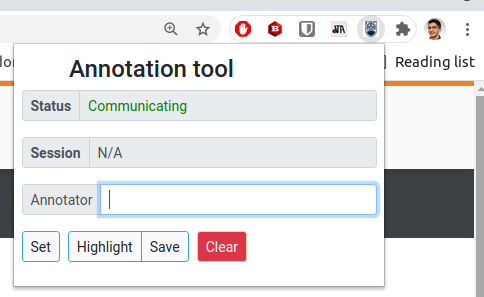
\includegraphics[width=\textwidth]{cp4/annotation-tool}
    \caption{Annotation tool and relevant sentences marked by an annotator}
    \label{fig:corpus-annotation-tool}
\end{figure}


\subsubsection{Results}

--- Provide summary of size of \acs{DS-android-small}. 

--- Descriptive statistics for marked sentences, similar to ICPC paper

--- State how the manually produced data can be used for the evaluation newly developed
techniques




\subsection{Automatic relevant text detection}
\label{cp4:relevant-text-auto}





We rely on state-of-the-art approaches~\cite{nadi2020, Robillard2015, Lotufo2012, Xu2017} able to automatically identify relevant text for a parcel of the  artifact types in our corpus, namely API documentation, GitHub issues, and Stack Overflow answers.
The text automatically identified by these approaches can serve as a baseline for 
any new technique applied to the same artifact types. 
To establish this baseline we use the text identified by human annotators and report the accuracy of the approaches we make use of.


\subsubsection{Automatic approaches}


To identify approaches applicable to the artifacts in our corpus, we systematically reviewed related work. We searched for approaches based on their availability in existing replication packages and their readiness for use.
We also refrained from using approaches with training procedures (e.g., ~\cite{liu2020} or ~\cite{Treude2016}) because of the challenges related to correctly tuning such supervised approaches~\cite{Chaparro2017, fucci2019}. Based on these criteria, three approaches were selected for the artifact sources in parenthesis:


\begin{itemize}[leftmargin=\parindent, font=\normalfont\itshape]
    \item \texttt{\acs{AnsBot}} (\textit{SO Answers}) uses several features (e.g., information entropy, textual patterns, entity overlap, etc.) to determine that a sentence has useful information to a developer's technical question~\cite{Xu2017}.
    
    \item \texttt{\acs{Krec}} (\textit{API Documentation}) identifies text fragments that reflect ``potentially important text that programmers cannot afford to ignore when using the API''~\cite{Robillard2015}.
    
    \item \texttt{\acs{Hurried}} (\textit{GitHub issues}) identify the most relevant sentences in a bug report based on three factors used to assess a sentence's relevancy (i.e., sentence's prominence in the issue, topic, and its similarity to the task)~\cite{Lotufo2012}.
\end{itemize}


\gm{I think you have to be clearer  that
Misc are included as non-annotated artifacts.}
\art{rephrased}

Due to the amount of variety in the content of miscellaneous sources, 
applying automatic approaches to detect relevant text for these types of artifacts
incurs the risk of using an approach for an artifact that the approach was not designed for.
Therefore, we refrain from using automatic approaches for miscellaneous artifacts.
With the exception of \acs{DS-android-small}, miscellaneous artifacts do not have associated task-relevant text detected and we leave this to future work.



% For the pertinent artifacts of our running example (Figure~\ref{fig:lock-screen-task}), 
% Tables~\ref{tbl:git-example-ansbot} to~\ref{tbl:git-example-hurried}
% illustrate sentences automatically detected by \acs{AnsBot}, \acs{Krec}, and \acs{Hurried}, respectively.
% \gm{Why give these three examples?}

 

% 
\begin{table}[H]
\centering    
\begin{scriptsize}
\begin{threeparttable}
\rowcolors{2}{}{lightgray}
\begin{tabular}{ll}

\hline
\multicolumn{2}{c}{\textit{How to add MediaPlayer controls on lock screen?}} \\
\hline
\hline

1 & \parbox[l][.8cm][c]{10.5cm}{I had the same problem, and well, the solution was simple, do not use any widget, simply use the RemoteControlClientCompat class.} \\
2 & \parbox[l][.8cm][c]{10.5cm}{Here is my lockScreenControls() method code, which I call whenever I want to show this type of control (when plays a song).} \\
3 & \parbox[l][.5cm][c]{10.5cm}{Thank @ianhlake for the good 2 video} \\

\hline


\end{tabular}
\end{threeparttable}
\end{scriptsize}
\caption{Pertinent sentences automatically detected by \acs{AnsBot}}
\label{tbl:git-example-ansbot}
\end{table}
% 
\begin{table}[H]
\centering    
\begin{scriptsize}
\begin{threeparttable}
\rowcolors{2}{}{lightgray}
\begin{tabular}{ll}
    
\hline
\multicolumn{2}{c}{\textit{Lock task mode - Android Developers}} \\
\hline
\hline

1 & \parbox[l][.8cm][c]{10.5cm}{You might use lock task mode if you're developing a kiosk application or a launcher to present a collection of apps.} \\
2 & \parbox[l][.8cm][c]{10.5cm}{To check if the current app is running in lock task mode, use the methods on ActivityManager as shown in the following example:} \\
3 & \parbox[l][.8cm][c]{10.5cm}{You can call KeyguardManager methods to find out if the device is locked and use an Activity lifecycle callback (such as onResume() that's called after unlocking) to start lock task mode.} \\
\hline

\end{tabular}
\end{threeparttable}
\end{scriptsize}
\caption{Pertinent sentences automatically detected by \acs{Krec}}
\label{tbl:git-example-krec}
\end{table}
% 
\begin{table}[H]
\centering    
\begin{scriptsize}
\begin{threeparttable}
\rowcolors{2}{}{lightgray}
\begin{tabular}{ll}

\hline
\multicolumn{2}{c}{\textit{How to add MediaPlayer controls on lock screen?}} \\
\hline
\hline

1 & \parbox[l][.8cm][c]{10.5cm}{I had the same problem, and well, the solution was simple, do not use any widget, simply use the RemoteControlClientCompat class.} \\
2 & \parbox[l][.8cm][c]{10.5cm}{Here is my lockScreenControls() method code, which I call whenever I want to show this type of control (when plays a song).} \\
3 & \parbox[l][.5cm][c]{10.5cm}{Thank @ianhlake for the good 2 video} \\

\hline


\end{tabular}
\end{threeparttable}
\end{scriptsize}
\caption{Pertinent sentences automatically detected by \acs{Hurried}}
\label{tbl:git-example-hurried}
\end{table}







\subsection{Accuracy}
\label{cp4:relevant-text-accuracy}

\gm{You need to get across that in applying
the techniques to this new data you need to
check if the results are similar to what was
reported for the technique authors. Doesn't
this require you to speak to whether the accuracy
is similar to what the authors reported for
the techniques?}

\vspace{3mm}
\art{I'm stuck here because of two potential result outcomes: similar results VS negative results.}



\vspace{3mm}
\gm{W}e apply a set of approaches 
to tasks and artifacts outside the ones where they were originally proposed and evaluated~\cite{nadi2020, Robillard2015, Lotufo2012, Xu2017}.
For instance, \acs{AnsBot}'s design was based on general Java programming tasks~\cite{Xu2017} while the tasks in our corpus comprise Android development and originate both from GitHub and from Stack Overflow. 
Likewise, \acs{Krec} was originally designed using the Java SE documentation~\cite{Robillard2015} 
while API documents in \acs{DS-android} comprise Android development\footnote{\url{https://developer.android.com/docs}}.
Because of such differences, we ask:


\begin{enumerate}[label={},leftmargin=0.7cm]
\item \textit{What is the accuracy of the approaches used to automatically detect text relevant in the task and artifacts in \acs{DS-android}?} 

\end{enumerate}


Answering this question will determine the portion of the text in \acs{DS-android} identified by an approach that 
is indeed relevant (i.e., precision) and how much 
of the relevant text an approach is able to detect (i.e., recall).
In turn, this information will help future research in understanding
how the automatically detected text in our corpus can be used in evaluation of new techniques for the automatic detection of relevant text. 




\subsubsection{Metrics}

To compute an approach's accuracy, we use standard \textit{precision} and \textit{recall} metrics~\cite{Manning2009IR} and the text marked by the human annotators in \acs{DS-android-small}.
Since the text marked by them varies, we compute metrics when the manually produced golden data consists of the text marked by one, two, or the three annotators (i.e., $n=1, 2,$ or $3$).

\gm{I am not quite following ratio here...}
\art{I removed references to ratio and started using accuracy}



To ease interpreting precision and recall, Table~\ref{tbl:type-I-II-errors} show all possible evaluation outcomes. The \textit{relevant} and \textit{not-relevant} columns represent the text 
marked (or not) by the annotators. Rows represent the text automatically identified by an automatic approach.


\begin{table}[H]
\centering    
\begin{scriptsize}
\begin{threeparttable}
\begin{tabular}{l|l|l}

\hline

\textbf{}
& \textbf{Relevant}    
& \textbf{Not-relevant} \\

\hline
\hline

\textbf{Identified as relevant} & true positive ($TP$) & false positive ($FP$) \\
\hline
\textbf{Identified as Not-relevant} & false negative ($FN$) & true negative ($TN$) \\
\hline

\end{tabular}
\end{threeparttable}
\end{scriptsize}
\caption{Result outcomes}
\label{tbl:type-I-II-errors}
\end{table}

    



For a given task $t$ and artifact $a$, $precision_n$ is the fraction of the sentences identified that are marked as relevant by $n$ annotators over the total number of sentences identified, as shown in Equation~\ref{eq:cp4:precision}. For example, \textit{precision(t, API documentation)\textsubscript{2}} computes the number of sentences identified by \acs{Krec} for the task $t$ when 
golden data consist of sentences marked by two or more annotators.


\begin{equation}
\label{eq:cp4:precision}    
    Precision(t, a)_n = \frac{TP}{TP + FP}
\end{equation}


Recall ($recall_n$) represents how many of all sentences marked by at least $n$ annotators are identified by a technique (Equation~\ref{eq:cp4:recall}).


\begin{equation}
\label{eq:cp4:recall}        
    Recall(t, a)_n = \frac{TP}{TP + FN}
\end{equation}

% \vspace{3mm}




% \subsection{Results}
% \textcolor{white}{force ident} % this is just for the chapter outline


% --- Discuss results.\footnote{\red{think which summary tables should I have in the thesis body and which I can move to Appendices}} \vspace{3mm}



% --- Precision~\ref{tbl:ds-small-results-precision}  \vspace{3mm}


% --- Recall~\ref{tbl:ds-small-results-recall} \vspace{3mm}

% --- Likely explanation for the results obtained.

% % When interpreting results, we favor precision instead of recall.
% % A false positives may contribute to a developer abandoning reading of an artifact that would otherwise provide crucial information for her task~\cite{Rastkar2010}.




% \begin{table}[H]
\centering    
\begin{scriptsize}
\begin{threeparttable}
\begin{tabular}{lcccccc}

\hline


\multirow{2.5}{*}{Technique}
& \multicolumn{2}{c}{\textit{$Precision_{n=3}$}}
& \multicolumn{2}{c}{\textit{$Precision_{n=2}$}}
& \multicolumn{2}{c}{\textit{$Precision_{n=1}$}}
\\ \cmidrule(l){2-3} \cmidrule(l){4-5} \cmidrule(l){6-7} 


& \textit{mean}
& \textit{std}
& \textit{mean}
& \textit{std}
& \textit{mean}
& \textit{std}
\\


\hline
\hline

\acs{AnsBot} 
& 0.5 & 0.5 % = 3
& 0.5 & 0.5 % = 2
& 0.5 & 0.5 % = 1
\\

\acs{Krec} 
& 0.5 & 0.5 % = 3
& 0.5 & 0.5 % = 2
& 0.5 & 0.5 % = 1
\\

\acs{Hurried} 
& 0.5 & 0.5 % = 3
& 0.5 & 0.5 % = 2
& 0.5 & 0.5 % = 1
\\

\hline

\end{tabular}
\end{threeparttable}
\end{scriptsize}
\caption{Precision of each technique for the tasks of \acs{DS-android-small}}
\label{tbl:ds-small-results-precision}
\end{table}

    

% \begin{table}[H]
% \centering    
% \begin{scriptsize}
% \begin{threeparttable}
% \begin{tabular}{lcccccccccccc}

% \hline


% \multirow{2.5}{*}{Technique}
% & \multicolumn{10}{c}{\textit{Tasks}} 
% & \multicolumn{2}{c}{\textit{Precision}}
% \\  \cmidrule(l){2-11} \cmidrule(l){12-13} 



% &
% \textit{T1} & \textit{T2} & \textit{T3} & \textit{T4} & \textit{T5}
% & \textit{T6} & \textit{T7} & \textit{T8} & \textit{T9} & \textit{T10}
% & \textit{mean}
% & \textit{std}
% \\


% \hline
% \hline

% \acs{AnsBot} 
% & 0.5 & 0.5 & 0.5 & 0.5 & 0.5
% & 0.5 & 0.5 & 0.5 & 0.5 & 0.5
% & 0.5 % mean
% & 0.5 % std
% \\

% \acs{Krec} 
% & 0.5 & 0.5 & 0.5 & 0.5 & 0.5
% & 0.5 & 0.5 & 0.5 & 0.5 & 0.5
% & 0.5 % mean
% & 0.5 % std
% \\

% \acs{Hurried} 
% & 0.5 & 0.5 & 0.5 & 0.5 & 0.5
% & 0.5 & 0.5 & 0.5 & 0.5 & 0.5
% & 0.5 % mean
% & 0.5 % std
% \\

% \hline

% \end{tabular}
% \end{threeparttable}
% \end{scriptsize}
% \caption{Precision of each technique for the tasks of \acs{DS-android-small}}
% \label{tbl:ds-small-results-precision}
% \end{table}

    

% \begin{table}[H]
\centering    
\begin{scriptsize}
\begin{threeparttable}
\begin{tabular}{lcccccc}

\hline


\multirow{2.5}{*}{Technique}
& \multicolumn{2}{c}{\textit{$Recall_{n=3}$}}
& \multicolumn{2}{c}{\textit{$Recall_{n=2}$}}
& \multicolumn{2}{c}{\textit{$Recall_{n=1}$}}
\\ \cmidrule(l){2-3} \cmidrule(l){4-5} \cmidrule(l){6-7} 


& \textit{mean}
& \textit{std}
& \textit{mean}
& \textit{std}
& \textit{mean}
& \textit{std}
\\


\hline
\hline

\acs{AnsBot} 
& 0.5 & 0.5 % = 3
& 0.5 & 0.5 % = 2
& 0.5 & 0.5 % = 1
\\

\acs{Krec} 
& 0.5 & 0.5 % = 3
& 0.5 & 0.5 % = 2
& 0.5 & 0.5 % = 1
\\

\acs{Hurried} 
& 0.5 & 0.5 % = 3
& 0.5 & 0.5 % = 2
& 0.5 & 0.5 % = 1
\\

\hline

\end{tabular}
\end{threeparttable}
\end{scriptsize}
\caption{Recall of each technique for the tasks of \acs{DS-android-small}}
\label{tbl:ds-small-results-recall}
\end{table}

    


% \subsection{Threats}
% \label{cp4:corpus-threats}

% --- \red{Argue that this is not a replication study but rather establishing thresholds} \vspace{3mm}

% --- Discuss threats \vspace{3mm}



